\section{Software Switches \glsentryshort{sdn}}
\label{sec:softSwitchs}

En las redes definidas por software, los software switches desempeñan un papel fundamental al permitir la virtualización y la gestión centralizada de las redes. Estos switches, a diferencia de los switches de hardware tradicionales, se implementan como software y se ejecutan en servidores convencionales. Un software switch en \gls{sdn}, en adelante \textit{softswitch}, es una entidad lógica que reside generalmente en una instancia virtual o en un servidor, y se comunica con el controlador \gls{sdn} para recibir instrucciones sobre cómo procesar los paquetes de datos que fluyen a través de la red. Al estar basados en software, estos switches pueden ser escalados y desplegados de manera flexible según las necesidades y demandas de la red. La principal ventaja de los \textit{softswitches} radica en su capacidad para adaptarse y responder de manera dinámica a las necesidades de la red. Pueden implementar diferentes funciones de red, como enrutamiento, conmutación, balanceo de carga y seguridad, a través de la instalación de reglas desde el controlador \gls{sdn}. \\
\\
% fig
\begin{figure}[ht]
    \centering
    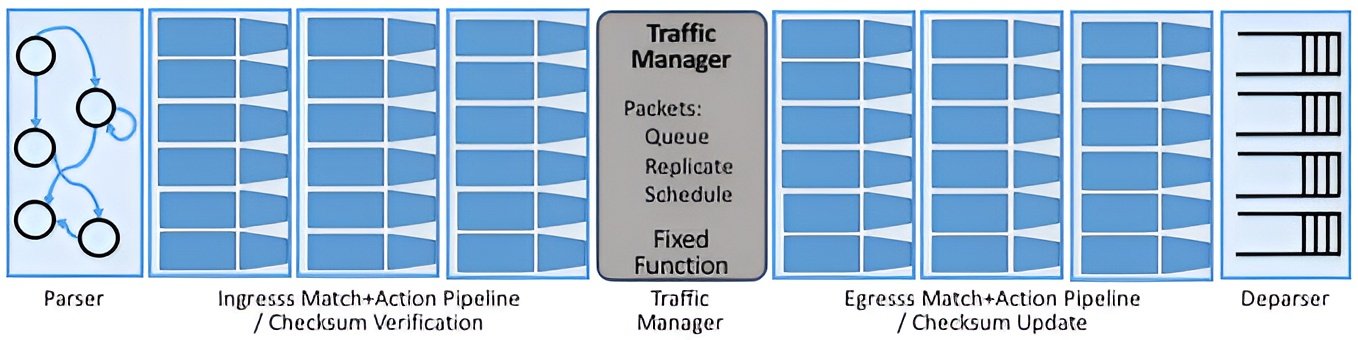
\includegraphics[width=0.8\textwidth]{archivos/img/teoria/softswitch.jpg}
    \caption{Arquitectura genérica de un \textit{softswitch} \gls{sdn} \cite{softswitches1}}
    \label{fig:softswitch}
\end{figure}

Según se puede apreciar en la figura \ref{fig:softswitch}, la arquitectura genérica de un \textit{softswitch} se puede resumir en los siguientes bloques. El primero de todos tiene que ser un parser, que vaya inspeccionando los paquetes entrantes a la pipeline de procesamiento del switch para identificar que tipo es. Una vez se ha identificado el paquete que se va a procesar, el siguiente bloque son las tablas de \textit{match-action}, las cuales tienen una interfaz de comunicación con el controlador \gls{sdn} para establecer criterios y campos de \textit{match}, y en caso de haber un \textit{match}, definir una serie de acciones para llevar a cabo. En función del \textit{softswitch}, la verificación de \textit{checksum}\footnote{Suma de comprobación, campo para comprobar la integridad del paquete de datos} se puede llevar a cabo en el parser o en la etapa de las tablas de \textit{match-action}. El siguiente bloque que nos podemos encontrar en un \textit{softswitch} es el conocido como gestor de tráfico, que variará en función de la implementación, pero nos proveerá de gestión de colas, \gls{qos}, duplicado de paquetes, etc. La siguiente etapa ya es más opcional, que se suele denominar como \textit{egress match-action}, la cual se puede utilizar para definir algún tipo de lógica a la salida de los switches, aunque en la realidad se suele utilizar para actualizar los campos  de \texttt{TTL} y recalcular el \textit{checksum} dado que el paquete se habrá visto modificado. El último bloque es el deparser, el cual se encarga de ensamblar de nuevo el paquete y prepararlo para sacarlo por el puerto de salida del switch.

\subsection{OvS}
\label{subsec:OVS}

\gls{ovs}, es uno de los \textit{softswitches} de referencia en el mundo de las redes, ampliamente utilizado tanto en la industria como en la academia. El switch está ofrecido como un proyecto opensource y respaldado por la Linux Foundation.  Es uno de los software switches más utilizados y ampliamente adoptados en entornos \gls{sdn} debido a su flexibilidad y funcionalidades avanzadas, aunque si tiene que destacar por algo, es por su gran rendimiento al trabajar a nivel de Kernel siendo idóneo para entornos de producción \cite{ovs1}. El \gls{ovs} actúa como un switch virtual, proporcionando capacidades de conmutación y reenvío para máquinas virtuales y contenedores en entornos de virtualización. Puede ejecutarse en hipervisores populares, como KVM (Kernel-based Virtual Machine), Xen y VMware, y también puede ser implementado como un switch independiente en instancias o servidores en modo standalone. Las características clave de Open vSwitch incluyen:

\begin{itemize}
    \item Agente \gls{sdn}: el switch ofrece una interfaz que permite que sea controlado mediante un controlador \gls{sdn}, como OpenDaylight o ONOS. Esto permite una gestión centralizada y un control más granular de la red, así como la implementación de políticas de red definidas por software.
    \item Funcionalidades avanzadas de alto rendimiento: \gls{ovs} ofrece una amplia gama de funcionalidades, como fast-forwarding al trabajar con frameworks como \gls{xdp}, DPDK o \gls{ebpf}. Estas características permiten una gestión eficiente de la red, y entorno de altas prestaciones ofreciendo un alto rendimiento perfecto para despliegues de producción.
    \item Integración con tecnologías de virtualización: \gls{ovs} se integra estrechamente con tecnologías de virtualización como OpenStack y Docker. Puede proporcionar conectividad de red entre máquinas virtuales, contenedores y hosts físicos, facilitando la migración y la gestión de recursos en entornos virtualizados.
    \item Extensibilidad y soporte para estándares: El \gls{ovs} es altamente extensible y se puede ampliar mediante la integración de módulos y complementos personalizados. Por ejemplo, para la integración del lenguaje de \gls{p4} se está haciendo de forma paulatina mediante módulos. Además, cumple con los estándares de la industria, como el protocolo OpenFlow, para garantizar la interoperabilidad con otros componentes \gls{sdn}.
\end{itemize}

Si nos fijamos en la figura \ref{fig:ovs}, podemos apreciar los componentes principales de la arquitectura del \gls{ovs}. Como se puede apreciar en la figura hay dos partes claramente diferenciadas en el \textit{softswitch}, una de espacio de usuario y otra parte de espacio de Kernel. Esta última es la que proveerá al \gls{ovs} de un alto rendimiento en comparación con otros software switches.  Los componentes principales del \gls{ovs} se pueden resumir en los siguientes puntos \cite{ovs1}.

\begin{itemize}
    \item \texttt{ovs-vswitchd}, es un \textit{daemon} que corre en espacio de usuario que implementa el switch, este proceso corre de forma conjunta con un módulo que corre en espacio de kernel, los cuales se comunican por netlink\footnote{\url{https://man7.org/linux/man-pages/man7/netlink.7.html}} para establecer la política de gestión de flujos.
    \item \texttt{ovsdb-server}, es un servidor de base de datos ligera, a la cual el proceso de espacio de usuario \texttt{ovs-vswitchd} le hace queries para obtener su configuración.
    \item \texttt{ovs-dpctl}, es una herramienta de gestión del módulo del kernel que implementa el datapath. El nombre de la herramienta hereda del nombre puesto a la herramienta original \texttt{dpctl}, la cual fue propuesta por Stanford en 2009\footnote{\url{https://github.com/mininet/openflow/blob/master/utilities/dpctl.c}}, y es un acrónimo de \textit{\textbf{d}ata\textbf{p}ath-\textbf{c}on\textbf{t}ro\textbf{l}}.
    \item \texttt{ovs-vsctl}, es uan utilidad para gestionar la configuración del proceso de espacio de usuario \texttt{ovs-vswitchd}.
    \item \texttt{ovs-appctl}, es una herramienta para mandar comandos a los \textit{daemon}s \gls{ovs}.
    \item \texttt{ovs-ofctl}, es una herramienta con la cual podemos mandar comandos y controlar vía OpenFlow el funcionamiento de switch.
    \item \texttt{ovs-testcontroller}, es un controlador experimental que implementan para testear la recepción y manejo de mensajes OpenFLow.
\end{itemize}

% fig
\begin{figure}[ht]
    \centering
    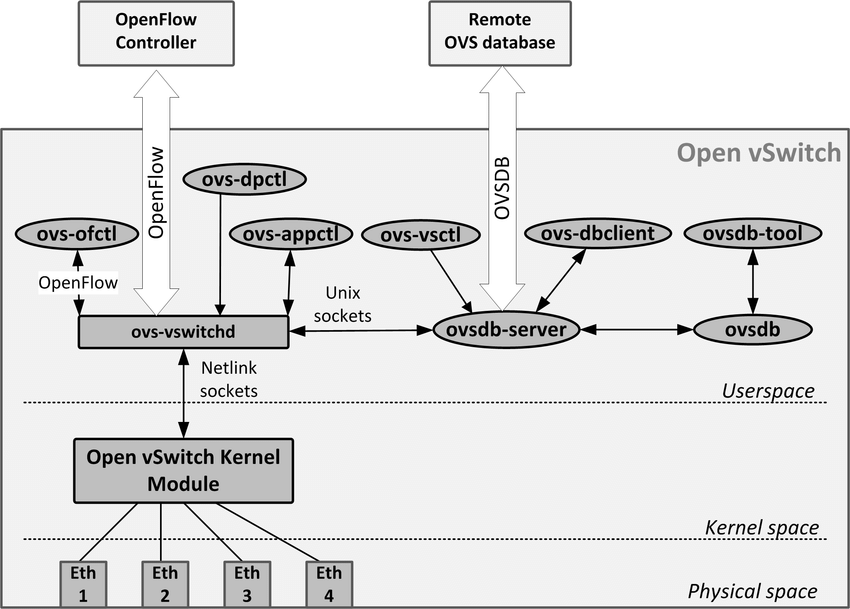
\includegraphics[width=0.7\textwidth]{archivos/img/teoria/ovs.png}
    \caption{Arquitectura del \glsentryshort{ovs} \cite{mendiola2016survey}}
    \label{fig:ovs}
\end{figure}

En resumen, el \gls{ovs} es un software switch \gls{sdn} ampliamente utilizado que proporciona capacidades avanzadas de conmutación y enrutamiento para entornos de virtualización. Su flexibilidad, funcionalidades avanzadas, rendimiento y compatibilidad con estándares lo convierten en una opción popular para implementaciones \gls{sdn} en diversos entornos, desde centros de datos hasta infraestructuras de proveedores de servicios.


\subsection{BOFUSS}
\label{subsec:BOFUSS}

\gls{bofus}, es la otra gran alternativa en el mundo de los software switches \gls{sdn}. Este switch nació como una primera implementación por el 2008 en la universidad de Stanford, acuñado como  \textit{The Stanford Reference OpenFlow Switch}. Esta implementación era un mínimo producto viable para demostrar y ayudar en el proceso de estandarización del protocolo \texttt{Openflow 1.0}. Dicho mínimo producto viable, fue retomado por los laboratorios de Ericsson, \textit{Ericsson Research TrafficLab}, para desarrollar la versión \texttt{Openflow 1.1}. \\
\\
Este último desarrollo fue retomado por el investigador Eder Leão Fernandes, desde el CPqD de Brasil, fue parte de su trabajo fin de máster y tesis doctoral, donde completo lo que hoy conocemos como el \gls{bofus}, el cual da soporte para la versión \texttt{Openflow 1.3}. Por último, se verá más adelante que este switch fue tomado por Boby Nicusor Constantin y modificado para hacer una implementación de control In-band. En la siguiente figura, ver figura \ref{fig:bofuss1}, se puede apreciar un pequeño resumen de la historia del software switch \gls{bofus}.

% fig
\begin{figure}[ht]
    \centering
    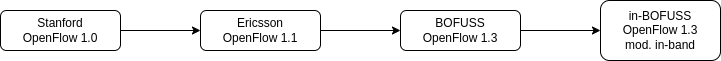
\includegraphics[width=\textwidth]{archivos/img/teoria/bofuss1.png}
    \caption{Evolución del \glsentryshort{bofus}}
    \label{fig:bofuss1}
\end{figure}

La arquitectura del \gls{bofus} se puede apreciar en la figura \ref{fig:bofuss2}. Según se ha podido averiguar, por el propio creador, esta arquitectura si bien es cierto que no trata de replicar la especificación de OpenFlow al $100\%$, es la implementación más cercana a la especificación oficial de \texttt{Openflow 1.3}. Como se puede ver en la figura siguiente (Figura \ref{fig:bofuss2}) , el software switch se compone de dos bloques fundamentales.

\begin{itemize}
    \item   Plano de datos, \textit{Datapath}, en la herramienta al plano de datos lo podemos encontrar como \texttt{udatapath/ofdatapath}.
    \item   Plano de control, \textit{Control plane}, en la herramienta al plano de control lo podemos encontrar como \texttt{secchan/ofprotocol}.
\end{itemize}

El primero de ellos, el \texttt{udatapath/ofdatapath} se caracteriza por ser el bloque funcional de gestionar el procesamiento de los paquetes datos, y en ocasiones de control (en función del paradigma de control). Dentro de este bloque funcional se pueden encontrar elementos internos como por ejemplo, los puertos, conocidos como \texttt{Port}, los \texttt{Flow}, \texttt{Meter}, \texttt{Group}, \texttt{Table} y el \texttt{Packet Parser}. El bloque del agente de control, es el encargado de gestionar la información de control entre el controlador y el dispositivo. Los mensajes de Openflow viajarán desde el plano de secure channel, a la librería de \texttt{oflib}, y de ahí al datapath para instanciar en las tablas de flujos correspondientes. Más adelante se explican en detalle cada bloque de la arquitectura.

% fig
\begin{figure}[ht]
    \centering
    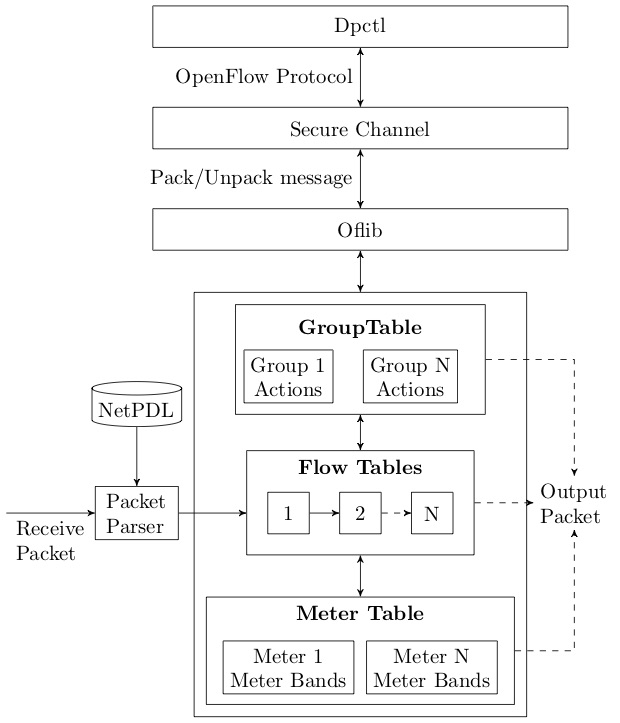
\includegraphics[width=0.8\textwidth]{archivos/img/teoria/bofuss2.png}
    \caption{Arquitectura del \glsentryshort{bofus}}
    \label{fig:bofuss2}
\end{figure}

\subsubsection{Ports}

Los puertos OpenFlow desempeñan un papel fundamental como puntos de entrada y salida para los paquetes de datos en un entorno OpenFlow. Cuando se ejecuta un software switch en una máquina, puede utilizar interfaces físicas o virtuales como sus puertos (interfaces físicas o virtuales como \gls{veth} o también radio taps emulados). Los puertos físicos permiten el control de interfaces Ethernet o WiFi, lo que facilita la gestión de tanto topologías de red realistas como emuladas. Aunque la velocidad del software switch puede ser limitada dado que trabaja en espacio de usuario, la posibilidad de crear un entorno de pruebas mejora la experiencia de los usuarios que desarrollan y evalúan aplicaciones OpenFlow. Se podría pensar que los puertos del switch se limitan simplemente a enviar y recibir paquetes de red, pero en verdad, también tienen una serie de responsabilidades relacionadas con la gestión del protocolo OpenFlow. Estas responsabilidades se pueden resumir en los siguientes puntos.

\begin{itemize}
    \item OpenFlow permite cierto nivel de control sobre el comportamiento que tiene que tener un puerto en particular. Si se recibe un mensaje de modificación de puerto, este tiene que permitir configurar el estado del puerto. Los puertos pueden configurarse para que descarten todos los paquetes recibidos, prohíban la generación de mensajes de tipo openflow \texttt{Packet-In} a partir de los paquetes que llegan, además de marcar el estado del puerto como fuera de servicio. El agente que gestione el puerto deben gestionar estos mensajes de configuración que le lleguen, y cambiar el comportamiento del puerto según la configuración recibida.

    \item Los puertos Openflow tienen que llevar un monitoreo del estado de la interfaz física o emulada que gestionan. Si bien es cierto que el controlador no puede actuar sobre el estado real de la interfaz, el switch tiene que informar sobre los cambios de estado del enlace.

    \item  Generalmente cuando se lleva a cabo un \texttt{Packet-In} porque hay un \textit{miss}, solo se manda al controlador las cabeceras del mensaje a consultar junto al propio mensaje del \texttt{Packet-In}. Los puertos, durante dicha consulta tendrán que gestionar los buffers que almacenarán los paquetes a consultar para ser procesados más tarde.

    \item El controlador a través del agente de control, también puede consultar sobre la descripción de un puerto. Por tanto, el software switch tendrá que recolectar la información que considere oportuna como por ejemplo la velocidad actual y máxima de las interfaces reales, almacenarla para enviarla posteriormente cuando el controlador se lo requiera.

    \item Las colas según se ha podido consultar no son parte de la definición estándar de Openflow. Sin embargo, Openflow puede  configurar colas asociadas a unos puertos dados. Los puertos por tanto tendrán la responsabilidad de llevar a cabo la asociación de configuración de cola y asociación de cola con un puerto además de actualizar los contadores de paquetes de puerto y cola asociada.
\end{itemize}

\subsubsection{Packet Parser}

Antes que el paquete en cuestión llegue a la pipeline de procesamiento del software switch, este debe ser procesado para adaptarlo a las estructuras de datos que se manejan en el switch. Para ello, el cómo se tiene que parsear los paquetes se definieron en el estándar de \texttt{OpenFlow 1.1}. Esto es importante, ya que debe haber consistencia en como los paquetes deben ser paserados, pero esto a su vez supuso una limitación para nuevos diseños de switches, y supone modificaciones cada vez que se añade un nuevo protocolo. Por ello, más adelante con especificaciones posteriores del protocolo esta limitación se vio eliminada. El parser que se tiene en el BOFUSS hace uso de \textbf{NetBee} como disector y parseador de paquetes. Una vez que se han identificado los campos de protocolo que contiene el paquete, se crea una estructura de matching con la cual se pasará a la pipeline de procesamiento del switch. A continuación, en la figura \ref{fig:bofuss3} se puede ver la estructura básica del parser.

% fig
\begin{figure}[ht]
    \centering
    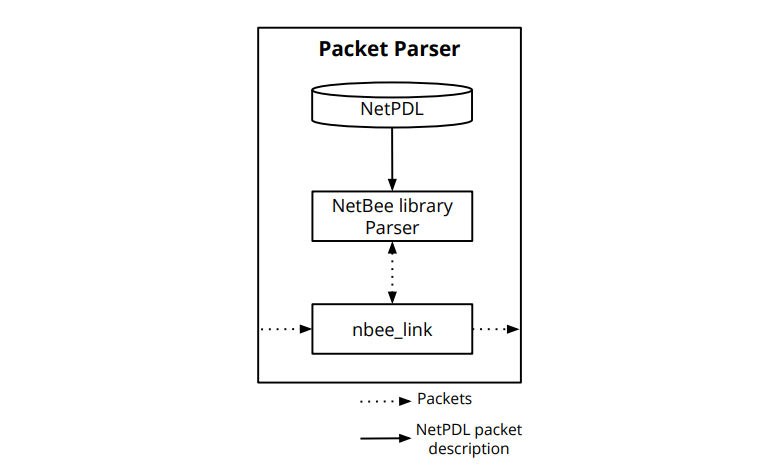
\includegraphics[width=\textwidth]{archivos/img/teoria/bofuss3.png}
    \caption{Parseador de paquetes del \glsentryshort{bofus}}
    \label{fig:bofuss3}
\end{figure}

Este paso de procesado del paquete anteriormente descrito se puede dar en dos ocasiones. A continuación se indican.

\begin{itemize}
    \item Que el paquete de red entre por uno de los puertos gestionados por el software switch.
    \item Que un paquete que ya ha sido modificado y redirigido por la pipeline de procesamiento, o enviado a una nueva tabla de adelante con la instrucción de \texttt{Go To Table}.
\end{itemize}

Esto se hace esta forma, dado que una revalidación del paquete es necesaria, y el parsear también se encarga de comprobar la validez del campo \texttt{TTL}. Además de añadir información de metadatos al mismo. Cada vez que se quiera dar soporte a nuevos protocolos, se tendrá que modificar el parsing del switch. Para ello, se tiene que llevar modificaciones a cabo en el fichero \texttt{*.xml} en lenguaje NetPDL. NetPDL es un lenguaje de descripción que describe cómo Netbee debe analizar los protocolos, la implementación actual del \gls{bofus} tiene su propio fichero ya creado, se puede consultar aquí\footnote{\url{https://github.com/NETSERV-UAH/in-BOFUSS/blob/main/customnetpdl.xml}}.

\subsubsection{Flow Tables}

Las \textit{Flow Tables} son el core de procesamiento del software switch. Las flow tables siempre son el siguiente paso después del procesamiento y podrían considerarse el corazón del entorno openflow dado que son el primer componente en la pipeline de procesamiento del switch. Aunque el uso de múltiples tablas de flujos es opcional, la especificación indica que se utilice al menos una tabla, a la hora de la implementación se considera más que recomendado, dado que, es inviable el hecho de gestionar el escalado de una aplicación con únicamente solo una tabla de flujo. \\
\\
En pocas palabras podríamos definir una  \textit{Flow Table} como una lista de flujos, donde cada flujo se compone de unos campos de matching y de unas instrucciones asociadas en caso de que haya match. Unas instrucciones que como se indican, tienen que estar definidas previamente en la especificación de Openflow. Una vez el paquete se ha validado y se ha parseado en una estructura de matching, se comprueba con una entrada de un flujo con el campo de matching, en caso de que coincida con dicho flujo, las instrucciones asociadas se ejecutan. A continuación, se indican algunos de los aspectos que tienen que cumplir las tablas de flujo.

\begin{itemize}
    \item La implementación de una tabla de \textit{miss} es obligatoria, ya que el switch tiene que hacer algo con los paquetes los cuales no coinciden con ninguna \textit{flow entry}. Por el contrario, si no se implementa ninguna tabla de \textit{miss}, se tiene que establecer una action por defecto. En el caso del switch, se ha establecido que se tiren los paquetes.

    \item Otro aspecto a considerar, el cual, tiene que ser gestionado por las \textit{Flow table} es la gestión de los paquetes \texttt{Flow-Mod}. Estos mensajes son generados desde el controlador y gestionados por el agente de control del switch para creación o eliminación de entradas de flujo en alguna \textit{Flow table}.

    \item El switch debe permitir al controlador de reconfigurar sus prestaciones. Es decir, las propiedades de las tablas deben ser conocidas por el controlador, y las tablas deben en todo momento responder a los mensajes de consulta de las características.

    \item Por cada paquete del plano de datos que les lleguen, deben llevar a cabo un \textit{look up},  es decir, consultar si el paquete entrante de datos coincide con algún campo de match de algún flujo de la tabla. En caso de que exista algún match, se ejecutará la instrucción asociada.

    \item  Otro aspecto a llevar a cabo por el switch, es llevar el recuento de las estadísticas de las entradas activas, los \textit{look ups} realizados, y paquetes que han hecho match.
\end{itemize}


En cuanto aspectos de implementación, podemos destacar, las reglas se indexan en las tablas de flujos en orden de prioridad, si tienen la misma prioridad, se indexarán en orden de llegada. En cuanto a la complejidad del tiempo de \textit{look up}, es lineal es decir $O(n)$, donde $n$ es el número de flujos. Esto no es muy eficiente, debido a que crece de forma lineal según el número de flujos aumenta. Aunque según ha indicado el autor, es suficiente para llevar pruebas de concepto, sin embargo, no es adecuado para un entorno industrial de producción. Otro detalle de implementación, que tenemos que tener en cuenta es el número de entradas de flujos por tabla de flujos, actualmente está definido a 64 por una macro.  Si se quisiera cambiar este parámetro solo habría que cambiar la macro y recompilar el proyecto. Por último, mencionar que las tablas de flujos tienen una lista de \texttt{idle} y \texttt{hard timeout}, que comprueban cada \texttt{100ms}, para ver si alguna de sus entradas de flujos han expirado.

\subsubsection{Group Table}

Las \textit{Group Tables}, se utilizan para agregar flow entries que tienen una política de acción similar. Cada grupo tiene un identificador único y contiene una lista de buckets que definen las acciones a tomar en caso de que el paquete coincida con ese grupo en particular. Cada bucket en una \textit{Group Tables} define una serie de acciones a ejecutar para un paquete que coincide con ese grupo. Estas acciones pueden incluir enrutamiento, reenvío a puertos específicos, encapsulación, copia de paquetes, descarte, entre otras. Un bucket puede tener múltiples acciones y también puede contener una acción especial para indicar que el paquete debe ser procesado por otros grupos en cascada. La utilización de \textit{Group Tables} permite un procesamiento más eficiente de los flujos de paquetes, ya que se pueden realizar acciones comunes de manera conjunta en lugar de procesar cada flujo de paquetes individualmente. Esto reduce la carga de procesamiento en los switches OpenFlow y facilita la implementación de políticas de red más complejas y flexibles. A continuación, en la figura \ref{bofuss4} se puede apreciar la estructura de las \textit{Group Tables}.

% fig
\begin{figure}[ht]
    \centering
    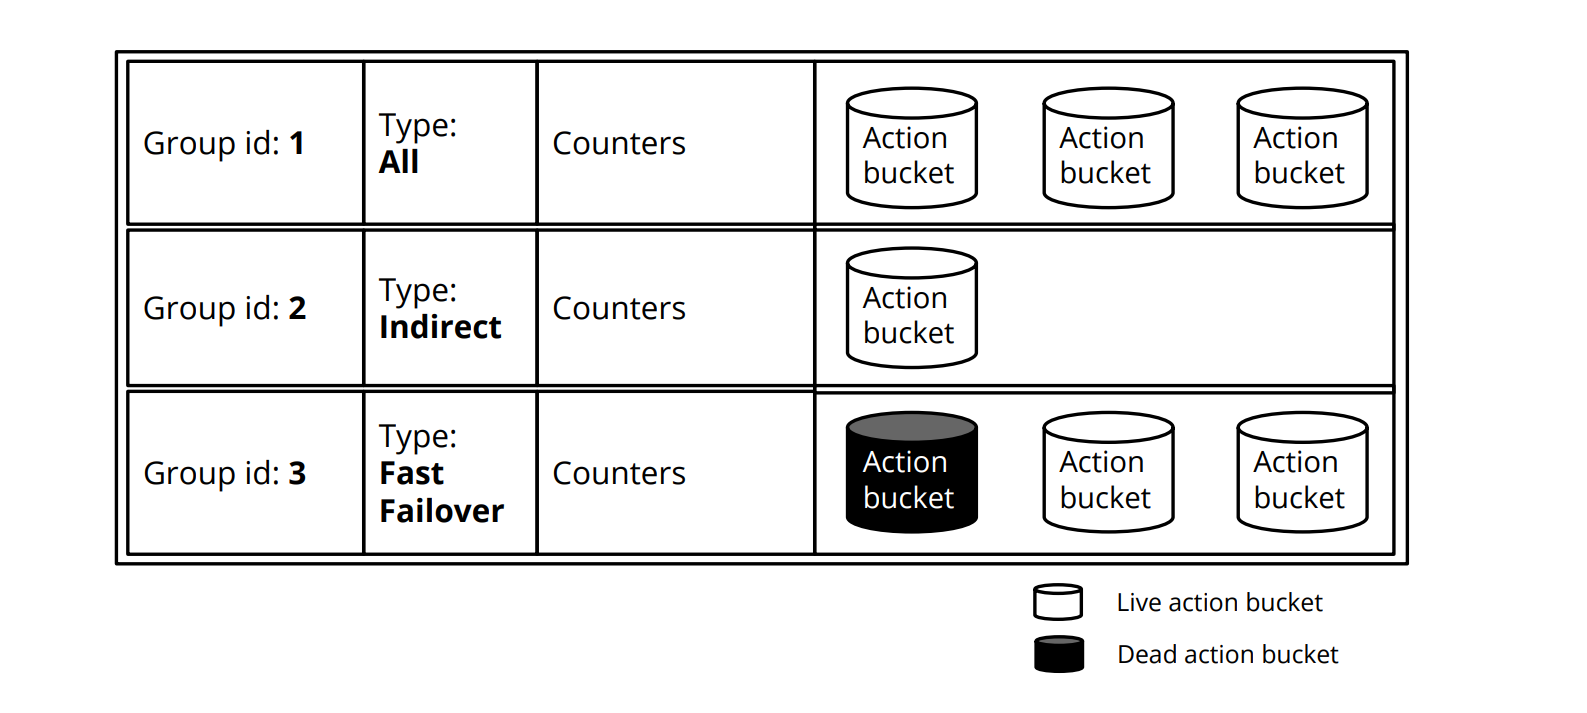
\includegraphics[width=\textwidth]{archivos/img/teoria/bofuss4.png}
    \caption{Estructura de las \textit{Group tables} del \glsentryshort{bofus}}
    \label{fig:bofuss4}
\end{figure}


\subsubsection{Meter Table}

La \textit{Meter Table} es el core del \gls{qos} del software switch. Para cada flujo se tienen unas meter asociadas en la propia entrada en la tabla de flujo. Dichas meters, tienen una entrada en la meter table. Cada entrada se compone de una ID, un contador, y unas meter bands. Estas últimas, las meters-bands son las encargadas de llevar a cabo las operaciones de \gls{qos}. Cada \textit{Meter Table} debe tener un tipo, un ratio, el cual será el límite que tiene que superarse para aplicar la action definida por el tipo de la meter. A continuación, se ver la figura \ref{fig:bofuss5} que ilustra la arquitectura de una Meter table.

% fig
\begin{figure}[ht]
    \centering
    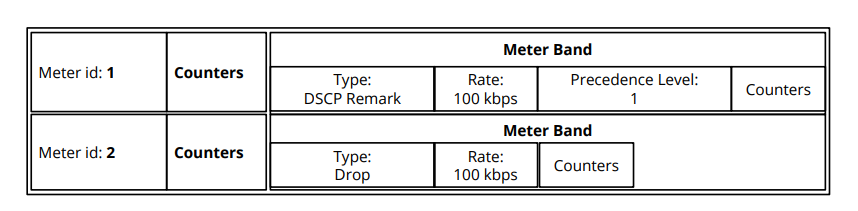
\includegraphics[width=0.8\textwidth]{archivos/img/teoria/bofuss5.png}
    \caption{Estructura de las \textit{Meter tables} del \glsentryshort{bofus}}
    \label{fig:bofuss5}
\end{figure}

Entre las responsabilidades de las meter tables podemos encontrarnos las siguientes:

\begin{itemize}
    \item Creación, destrucción y modificación de las entradas de las meters
    \item Medir el ratio de aquellos paquetes que han matchado en una flow entry, y apuntan a una meter table.
    \item Mantener actualizado los contadores de las estadísticas de los paquetes procesados por cada entrada en la meter table.
\end{itemize}

\subsubsection{oflib}

Los mensajes de OpenFlow están definidos de una manera en particular para ser transmitidos por la red. Los mensajes tienen que estar en modo 8-byte alineados, por lo que habrá alguna ocasión donde se tenga que añadir padding para que se cumpla esta regla. Otro requisito es que el mensaje tiene que estar en Network byte order, es decir, Big Endian. Los mensajes OpenFlow que se mandan por la red tienen que estar en el formato indicado anteriormente, es decir, el byte de mayor peso de una palabra tiene que estar almacenado en la posición más pequeña (la dirección más baja).

% fig
\begin{figure}[ht]
    \centering
    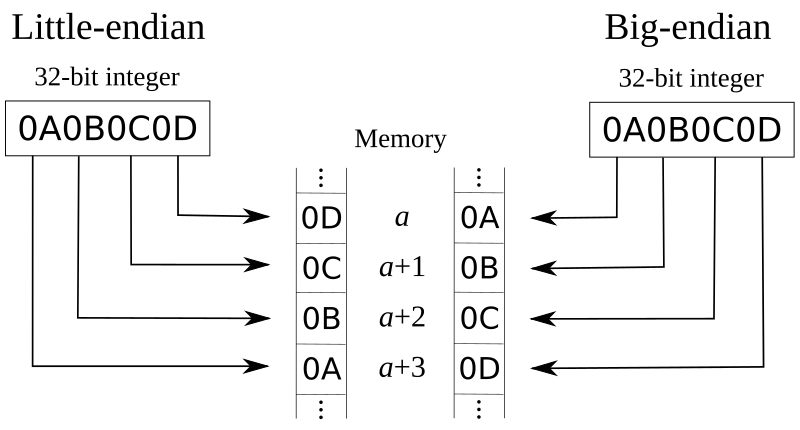
\includegraphics[width=0.8\textwidth]{archivos/img/teoria/bofuss6.png}
    \caption{Proceso de Marshaling y Unmarshaling }
    \label{fig:bofuss6}
\end{figure}

Las arquitecturas de cada máquina pueden variar, y el formato de datos con en el que trabajan también. Por ejemplo para ARM e Intel el formato con el cual trabajan ambas arquitecturas es Little Endian byte order. Por ello, en aras de manejar y codificar mensajes openflow se requiere una conversión big-endian a little-endian. Debido a cuál, se necesita una capa de abstración de la arquitectura donde se vaya a correr dicho software switch. Por ello, aunque el estándar de Openflow no lo indique, se ha añadido esta librería denominada como \texttt{oflib}. La función principal de esta librería es las operaciones de  marshaling y unmarshaling de los mensajes OpenFlow. Para que la transmisión de información de mensajes Openflow a la red se lleve a cabo de forma completamente autónoma. Las responsabilidades de esta librería por tanto son las siguientes.

\begin{itemize}
    \item Cada mensaje openflow debe tener una función para empaquetarlo y desempaquetarlo. De aquí en adelante, y en el repositorio, nos referimos a hacer un \textit{pack} es coger una estructura de datos openflow y prepararla para ser transmitida por la red. Cuando realizamos una operación de \textit{unpack}, cogemos información que viene por la red, y la convertimos a estructuras que entienda la arquitectura sobre la cual está corriendo nuestro software switch.
    \item Otra responsabilidad que tiene la librería es señalar con errores o warnings en caso de los mensajes Openflow estén mal codificados.
\end{itemize}


\subsubsection{Communication Channel}

El software switch se comunica con el controlador \gls{sdn} a través de este agente de control que actúa de proxy entre el datapath y el controlador \gls{sdn}. Este agente se encarga de gestionar las conexiones con el controlador \gls{sdn}, aunque, si bien es cierto que este agente no está pactado en el estándar de Openflow, esto da libertad a las diferentes implementaciones para configurar la conexión hacia al controlador como quieran. Por ejemplo, si se quiere que la conexión sea segura extremo a extremo, se tendría que utilizar TLS encima de TCP. Esta libertad de diseño en el canal de comunicación con el controlador, habré un \textit{gap} que se puede utilizar para desarrollar implementaciones dispares que ofrezcan distintas bondades y funcionalidades. Entre las responsabilidades de esta capa podemos mencionar las siguientes.

\begin{itemize}
    \item El agente de control se tiene que encargar de abrir una conexión TCP entre el switch y el controlador.
    \item El establecimiento de la conexión es responsabilidad del agente de control. Después del inicio de la conexión, el switch negocia la versión Openflow a utilizar entre el switch y el controlador. Este proceso se conoce como handshake.
    \item El agente de control debe soportar más de un controlador.
    \item Además, el agente de control debe soportar más de una conexión con el mismo controlador.
\end{itemize}